\documentclass{article}

\usepackage{amsmath}
\usepackage{amsthm}
\usepackage{amssymb}
\usepackage{bbm}
\usepackage{fancyhdr}
% \usepackage{listings}
\usepackage{cite}
\usepackage{graphicx}
\usepackage{enumitem}
\usepackage{courier}
\usepackage[pdftex,colorlinks=true, urlcolor = blue]{hyperref}

\oddsidemargin 0in \evensidemargin 0in
\topmargin -0.5in \headheight 0.25in \headsep 0.25in
\textwidth 6.5in \textheight 9in
\parskip 6pt \parindent 0in \footskip 20pt

% set the header up
\fancyhead{}
\fancyhead[L]{Stanford Aeronautics \& Astronautics}
\fancyhead[R]{Fall 2020}

%%%%%%%%%%%%%%%%%%%%%%%%%%
\renewcommand\headrulewidth{0.4pt}
\setlength\headheight{15pt}

\usepackage{xparse}
\NewDocumentCommand{\codeword}{v}{%
\texttt{\textcolor{blue}{#1}}%
}

\usepackage{xcolor}
\setlength{\parindent}{0in}

\title{AA 274A: Principles of Robot Autonomy I \\ Final Project Checkin}
\author{Group 30 \\ Parthiv Krishna, Shawn Manuel, Mason Llewellyn, Li Khoo}
\date{}

\begin{document}

\maketitle
\pagestyle{fancy} 

\section*{Finite State Machine}
Below is our FSM diagram. The top diagram is the higher level FSM showing the explore mode and the delivery loop. The bottom diagram is the drive mode FSM, which applies during the \codeword{Drive:Explore} (with dynamically generated goal positions), \codeword{Drive:Vendor}, and \codeword{Drive:Orderer} states. It handles the trajectory following, pose stabilization, and stopping and restarting at stop signs. 
\begin{center}
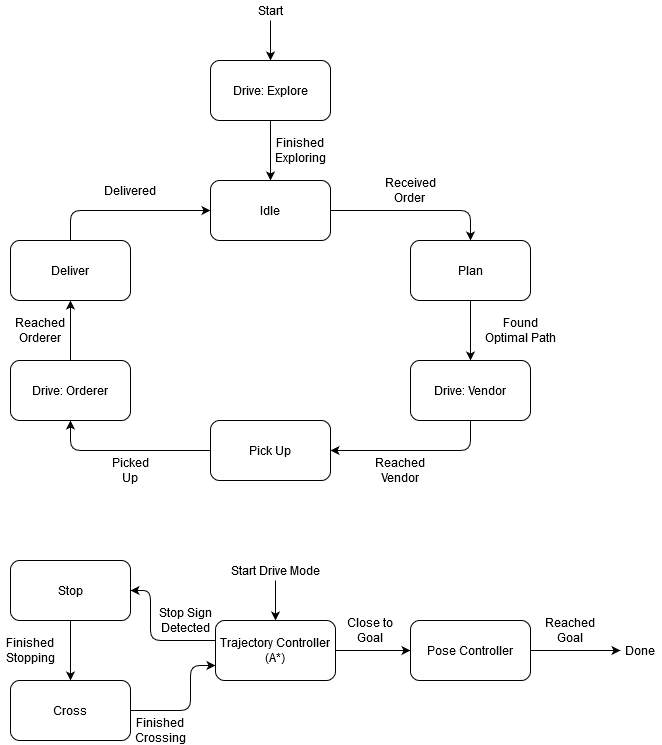
\includegraphics[width=0.75\textwidth]{fsm.png}
\end{center}

\section*{Extensions}
We intend to do the following extensions:
\begin{enumerate}
    \item Our robot will autonomously explore its environment without any human input. It will use this exploration phase to locate the different vendors.
    \item Our robot will stop at stop signs that are scattered throughout the map for a few seconds before continuing. We intend to use the CNN coupled with LIDAR to locate the stop signs and stop a certain (yet untuned) distance from them. 
    \item Our robot will accurately localize itself in its environment with Monte Carlo Localization/particle filtering. 
    \item We will have more vendor locations (6-8) than food types (3-4). Just before or at the time of launch, the distributions of foods among the vendors will be randomized. During the autonomous exploration phase (extension 1), the locations and food types of each vendor will be discovered using the CNN. When an order is placed for a specific type of food, it will also associated with a specific delivery location (specified at the time of order to be anywhere in the world that the orderer wants). The robot will determine the vendor for that type of food that would result in the shortest total drive distance (current location $\xrightarrow{}$ vendor $\xrightarrow{}$ delivery), then drive to that vendor and deliver the food to the specified location.
    
    
    
\end{enumerate}

\end{document}
